\section{Durchführung}
\label{sec:Durchführung}

\begin{figure}
    \centering
    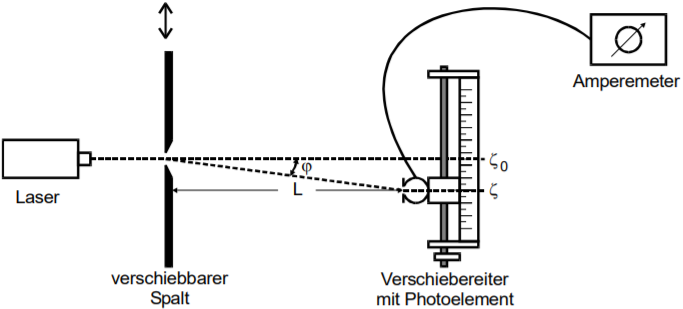
\includegraphics[width=\textwidth]{data/aufbau.png}
    \caption{Schematischer Aufbau des Versuchs.}
    \label{fig:aufbau}
\end{figure}

Für die Messung der Lichtintensität wird der Versuch wie in der schematischen Darstellung in Abb \ref{fig:aufbau} aufgebaut. Der 
lichtempfindliche Detektor befindet sich dabei $\SI{82.5}{\centi\metre} $ von dem Parallelspalt entfernt. Der Detektor wird so positioniert, 
dass zu Anfang der Messung möglichst das Intensitätsmaximum gemessen wird. Von da aus wird der Detektor an seiner präzise verschiebbaren 
Befestigung in $\SI{0.5}{\milli\metre} $ Schritten verschoben, bis das zweite Intensitätsminimum erreicht ist. Danach wird der Detektor
wieder zum Ursprünglichen Ort gesetzt und von da aus in gleichen Schritten in die andere Richtung vom absoluten Maximum weg verschoben, 
bis auch auf dieser Seite das zweite lokale Minimum erreicht ist. 
%Was wurde gemessen bzw. welche Größen wurden variiert?